\chapter{Appendices}
\section{Appendix A Network definition code}
\label{appendix:network_code}

\lstinputlisting[label=network_code_1,basicstyle=\scriptsize\ttfamily,caption=Network definition Python code]{code/network.py}

\cleardoublepage
\section{Appendix B Loss function code}
\label{appendix:loss_code}

\lstinputlisting[label=loss_code_1,basicstyle=\scriptsize\ttfamily,caption=Loss function Python code]{code/loss.py}

\cleardoublepage

\section{Appendix C Collage images}

\begin{figure}[b!]
    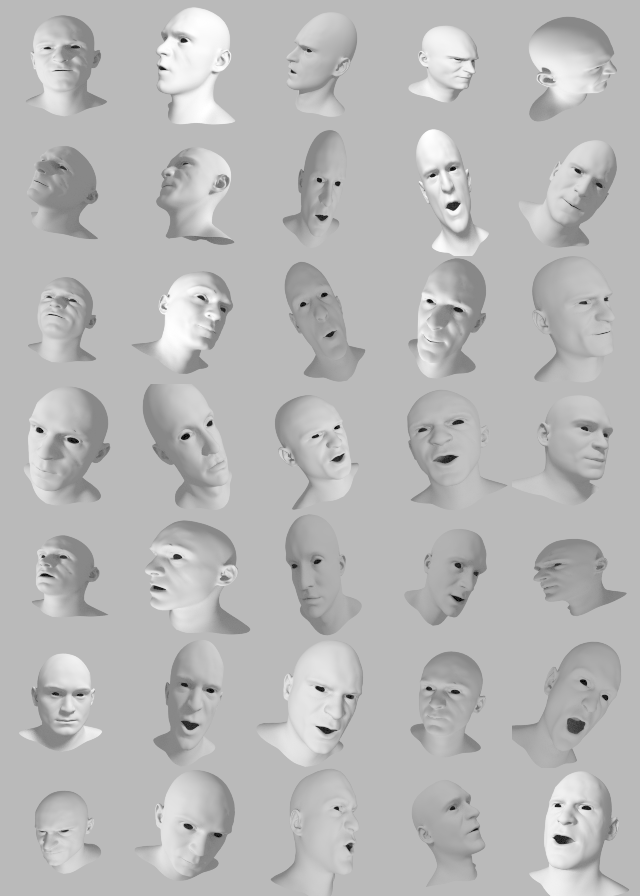
\includegraphics[width=\textwidth]{head_gray_collage}
    \caption[Gray head render collage]{A collage of head renders with gray textures. These were the most simplistic version of the head renders we used to train the network.}
    \label{fig:head_gray_collage_1}
\end{figure}

\begin{figure}
    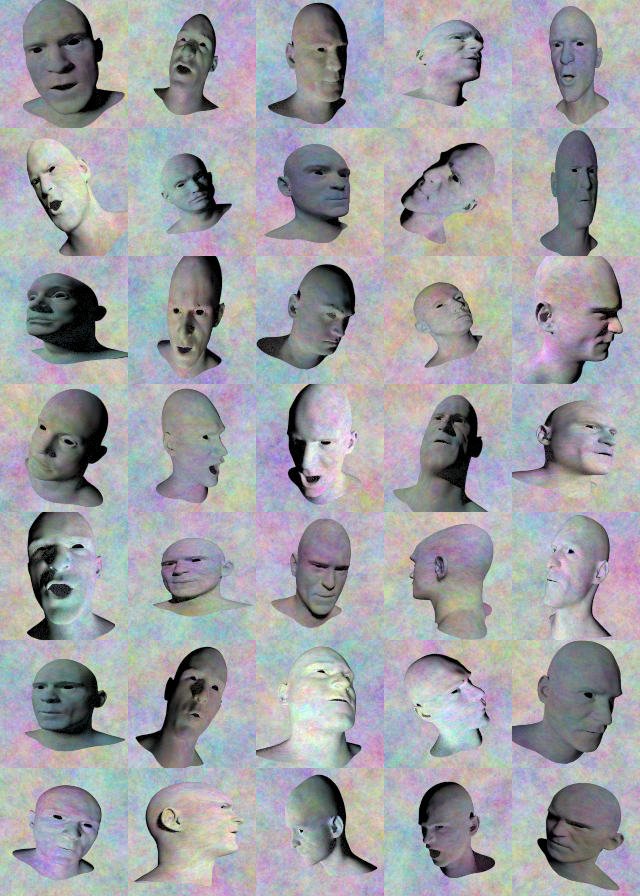
\includegraphics[width=\textwidth]{head_noise_collage}
    \caption[Noise head render collage]{A collage of head renders with 1/f noise textures. The 1/f noise should follow the power spectra of natural images. These or the gray head renders in figure \ref{fig:head_gray_collage_1} did not make the network generalize well to real-world images.}
    \label{fig:head_noise_collage_1}
\end{figure}

\begin{figure}
    
\includegraphics[width=\textwidth]{dummy2}
    \caption*{}
\end{figure}

\begin{figure}
    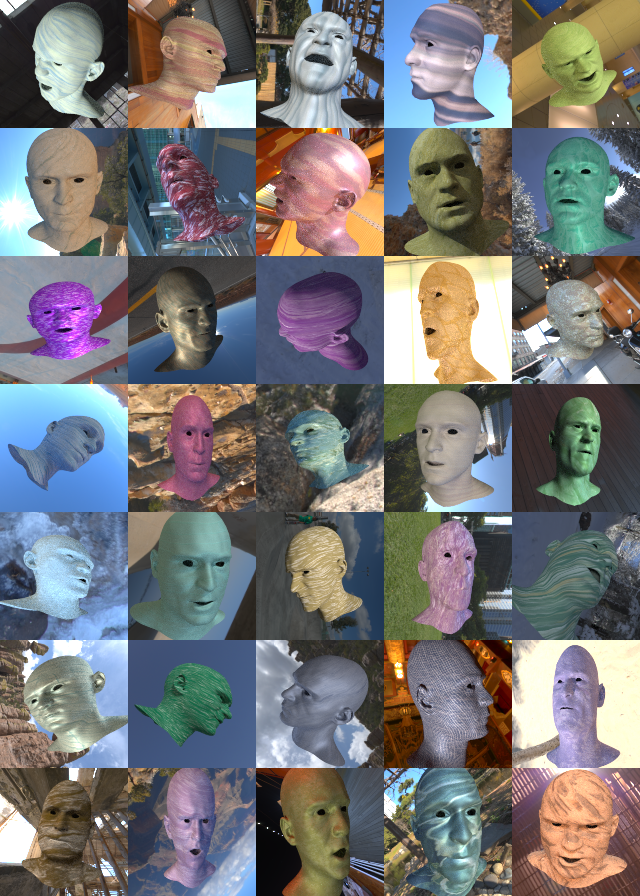
\includegraphics[width=\textwidth]{head_material_texture_collage}
    \caption[Non-realistic head render collage]{A collage of head renders with realistic background and non-realistic face textures. Surprisingly, a network trained with images like these performed similarly compared to a network trained with realistic face textures.}
    \label{fig:head_material_texture_collage_1}
\end{figure}

\begin{figure}
    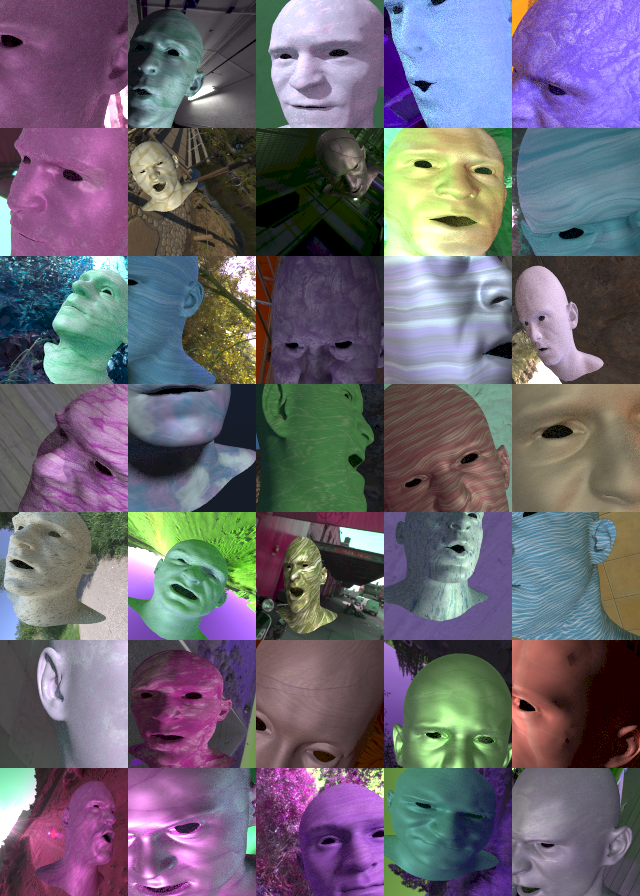
\includegraphics[width=\textwidth]{head_augment_shuffle_collage}
    \caption[Shuffle augmentation collage]{A collage of shuffle augmentations only. This augmentation increased the effective size of the training dataset by a factor of six. The same, non-augmented, image collage can be seen in figure \ref{fig:head_final_texture_collage_1}.}
    \label{fig:head_augment_shuffle_collage_1}
\end{figure}

\begin{figure}
    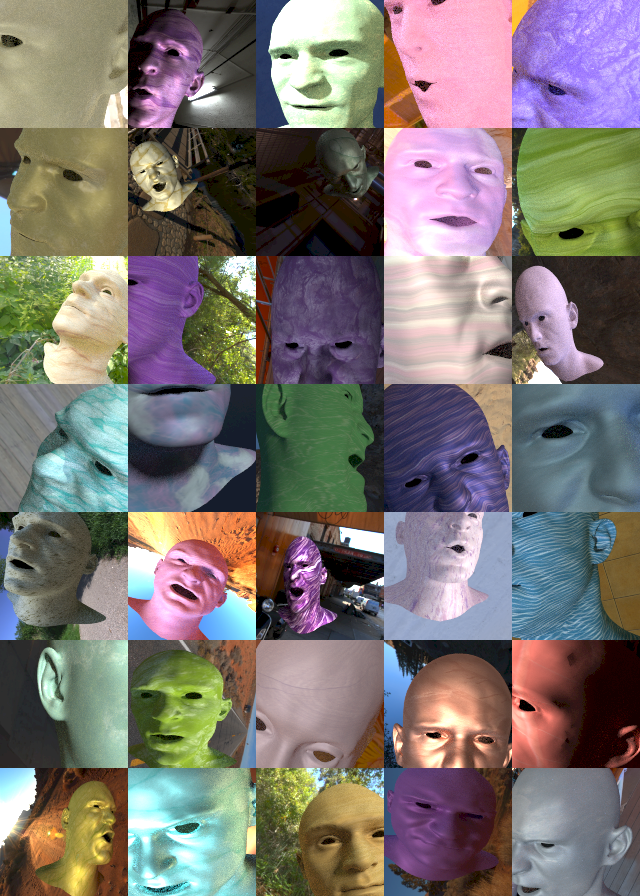
\includegraphics[width=\textwidth]{head_augment_expgamma_collage}
    \caption[Exposure and gamma augmentation collage]{A collage of exposure and gamma augmentations only. The variation in image brightness is more evident when compared with the same, non-augmented, image collage in figure \ref{fig:head_final_texture_collage_1}.}
    \label{fig:head_augment_expgamma_collage_1}
\end{figure}

\begin{figure}
    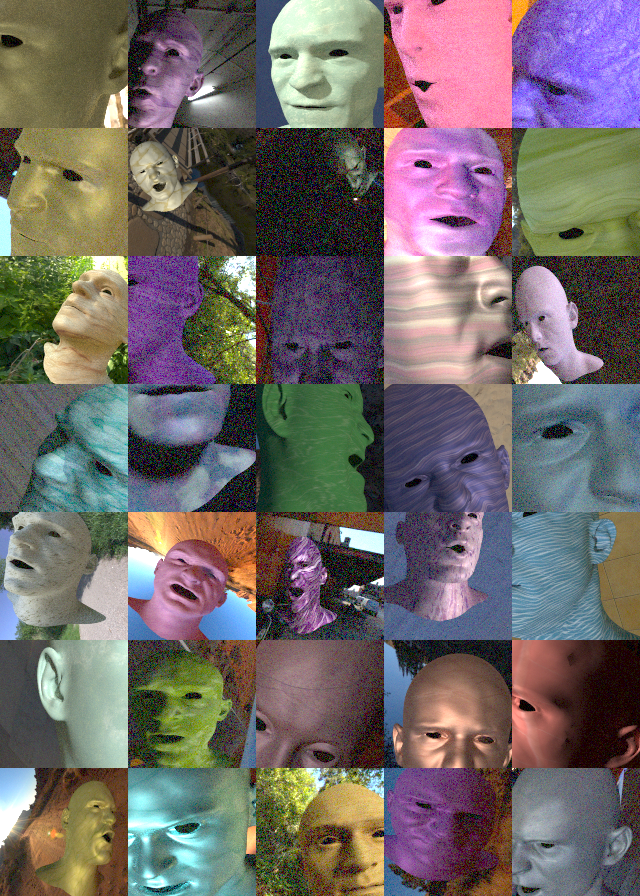
\includegraphics[width=\textwidth]{head_augment_noise_collage}
    \caption[Noise augmentation collage]{A collage of noise augmentations only. Noise augmentation like this helped the training process and made the network generalize better to real-world images. The noise is more evident when compared with the same, non-augmented, image collage in figure \ref{fig:head_final_texture_collage_1}.}
    \label{fig:head_augment_noise_collage_1}
\end{figure}

\begin{figure}
    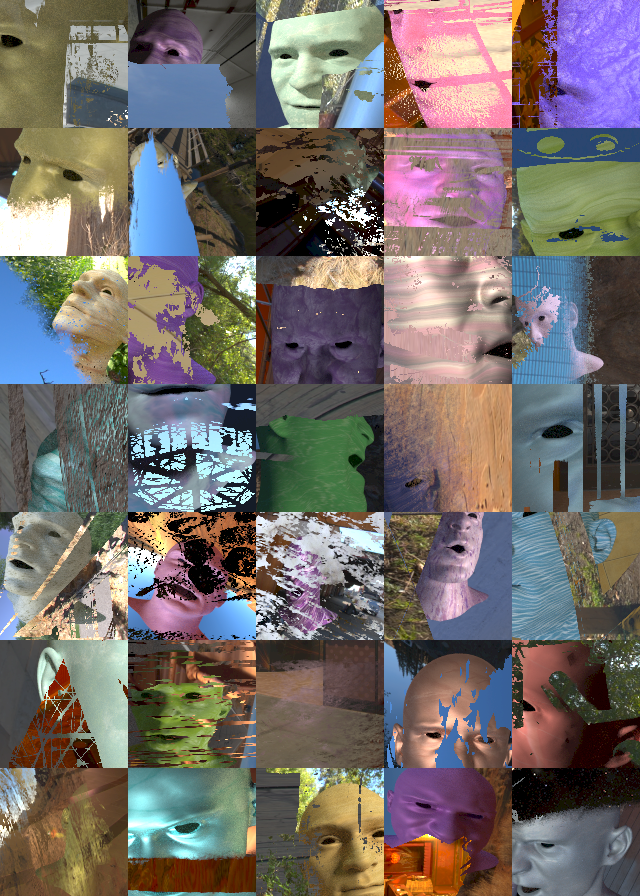
\includegraphics[width=\textwidth]{head_augment_occlusion_collage}
    \caption[Occlusion augmentation collage]{A collage of occlusion augmentations only. By using occlusion masks generated from realistic textures, we were able to make the network detect arbitrary occlusions and inpaint geometry underneath them. This image collage can be compared with the same, occlusion-free, image collage in figure \ref{fig:head_final_texture_collage_1}.}
    \label{fig:head_augment_occlusion_collage_1}
\end{figure}

\begin{figure}
    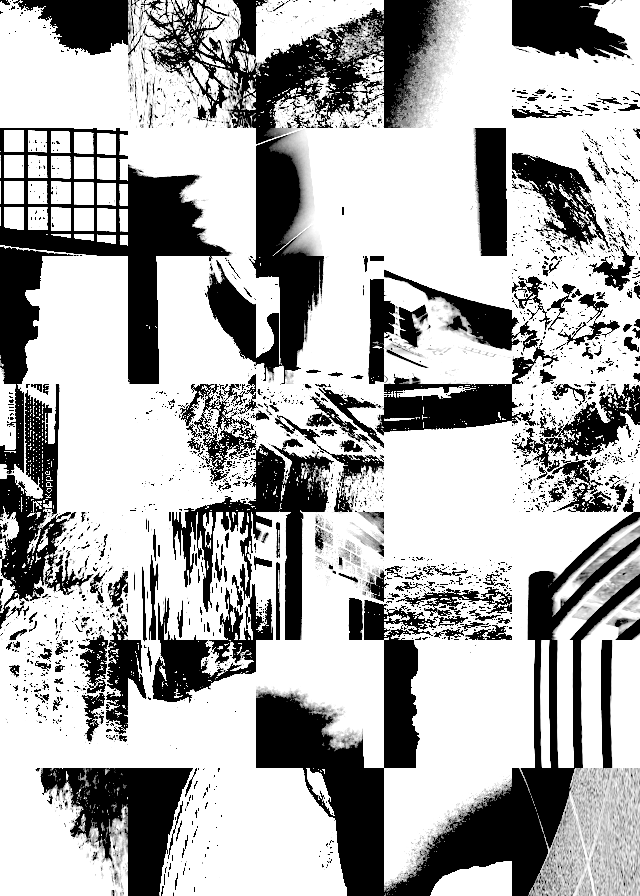
\includegraphics[width=\textwidth]{occlusion_mask_collage}
    \caption[Occlusion mask collage]{A collage of occlusion masks. These masks were used in the occlusion creation process depicted in figure number \ref{fig:occlusion_gen_1}. The mask generation method was adjusted so that the ratio of white-to-black pixels was visually about 50/50 in larger scale.}
    \label{fig:occlusion_mask_collage_1}
\end{figure}
